% vim:ft=tex:
%
\documentclass[class=article,border=1pt]{standalone}
\usepackage{amsmath}

\usepackage{tikz}
\usepackage{tikz-3dplot}
\usetikzlibrary{3d,shadings}
\usepackage{pgfplots}
\pgfplotsset{compat=1.11}
\usepackage[cm]{sfmath}
\renewcommand{\familydefault}{\sfdefault}

\begin{document}
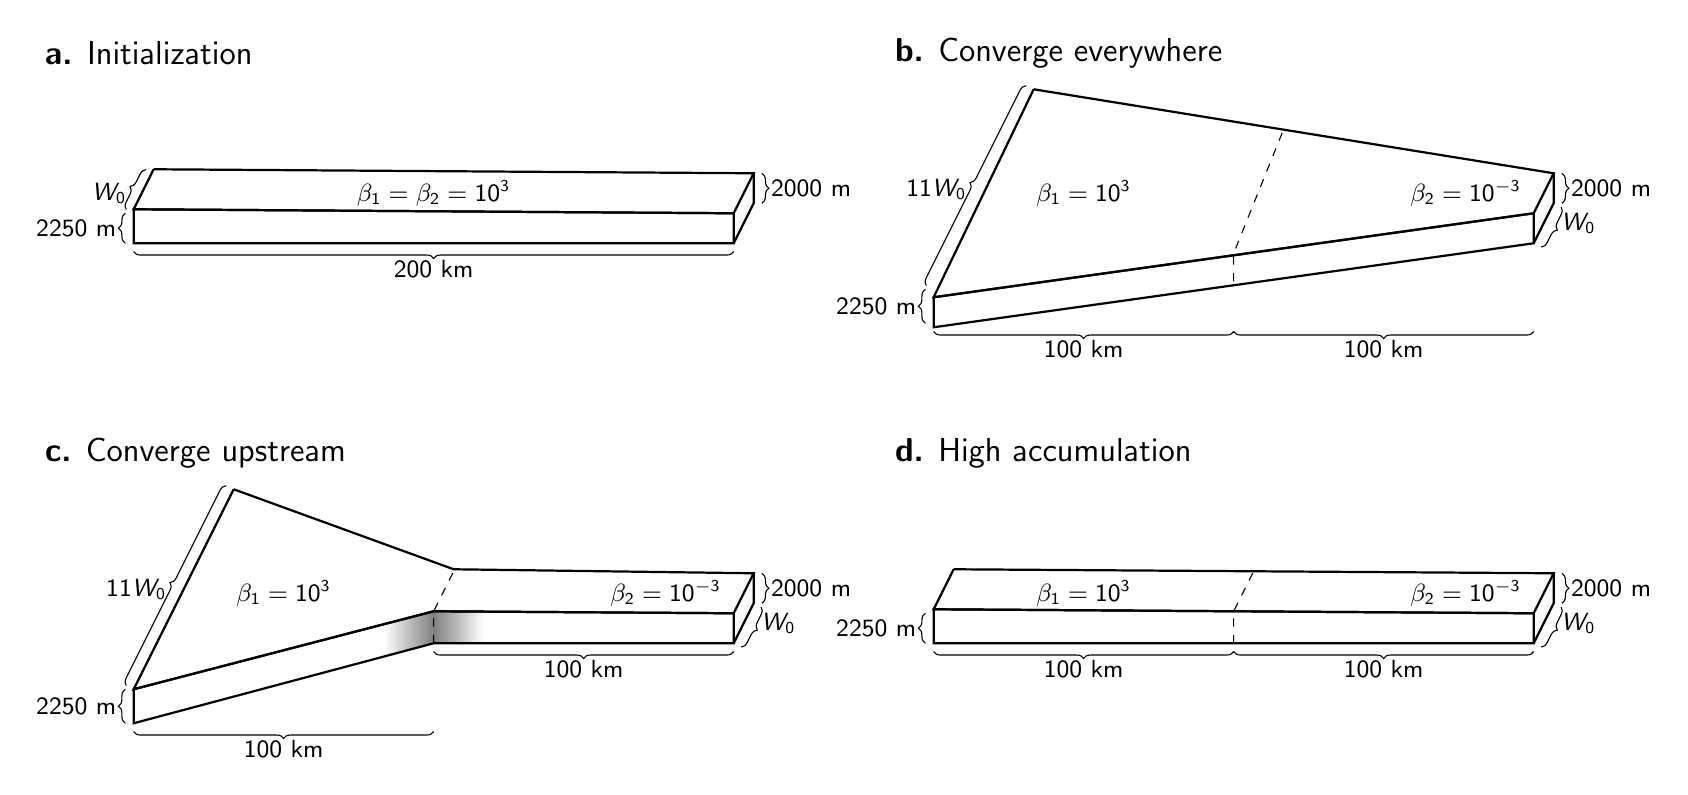
\begin{tikzpicture}[x=1in,y=1in]
    {\large
\node[right](A) at (-0.5, 0.7){{\bf a.} Initialization}; 
\node[right](B) at (3.75, 0.7){{\bf b.} Converge everywhere}; 
\node[right](C) at (-0.5, -1.3){{\bf c.} Converge upstream}; 
\node[right](D) at (3.75, -1.3){{\bf d.} High accumulation}; 
}
\small
\draw[thick, black] (0.1, 0.12) -- (1.6, 0.11) -- (3.1, 0.1)-- (3.0,-0.1)--(1.5, -0.09)--(0.0,-0.08)--(0.1, 0.12);
\draw[thick, black] (3.0,-0.1)--(1.5, -0.09)--(0.0,-0.08)--(0.0, -0.25)--(1.5,-0.25)--(3.0, -0.25)--(3.0,-0.1);
\draw[thick, black] (3.0, -0.25)--(3.1,-0.05)--(3.1,0.1);
% \draw[thin,black,dashed] (1.5, -0.25)--(1.5,-0.09)--(1.6,0.11);
\node(C3) at (1.5, 0.0){$\beta_1=\beta_2=10^3$}; 

% \shade[left color=gray, right color=white, shading angle=285] (5.25, -0.34)--(5.5, -0.31)--(5.5, -0.46)--(5.25, -0.5)--cycle;
% \shade[left color=gray, right color=white, shading angle=105] (5.75, -0.28)--(5.5, -0.31)--(5.5, -0.46)--(5.75, -0.42)--cycle;
% \shade[left color=red, right color=white, shading angle=-115] (6.25, -0.08)--(6.0, -0.14)--(6.15, 0.17)--(6.35, 0.12)--cycle;
% \shade[left color=red, right color=white, shading angle=75] (6.25, -0.08)--(6.5, -0.09)--(6.6, 0.12)--(6.35, 0.12)--cycle;
\draw[thick, black] (4.5, 0.52) -- (7.1, 0.1)-- (7.0,-0.1)--(4.0,-0.52)--(4.5, 0.52);
\draw[thick, black] (7.0,-0.1)--(4.0,-0.52)--(4.0, -0.67)--(7.0,-0.25)--(7.0,-0.1);
\draw[thick, black] (7.0, -0.25)--(7.1,-0.05)--(7.1,0.1);
\draw[thin,black,dashed] (5.5, -0.44)--(5.5,-0.30)--(5.75,0.32);

\node(C3) at (4.75, 0.0){$\beta_1=10^3$}; 
\node(C0) at (6.66, 0.0){$\beta_2=10^{-3}$}; 


\draw[decoration={brace,mirror,raise=3pt},decorate]
  (0,-0.25) -- node[below=3pt] {200 km} (3.0,-0.25);
\draw[decoration={brace,raise=3pt},decorate]
  (0,-0.1) -- node[left=3pt] {$W_0$} (0.1,0.1);
\draw[decoration={brace,raise=3pt},decorate]
  (0,-0.25) -- node[left=3pt] {2250 m} (0.0,-0.1);
\draw[decoration={brace,mirror,raise=3pt},decorate]
  (3.1,-0.05) -- node[right=3pt] {2000 m} (3.1,0.1);

\draw[decoration={brace,mirror,raise=3pt},decorate]
  (4.0,-0.65) -- node[below=3pt] {100 km} (5.5,-0.65);
\draw[decoration={brace,mirror,raise=3pt},decorate]
  (5.5,-0.65) -- node[below=3pt] {100 km} (7.0,-0.65);
\draw[decoration={brace,mirror,raise=3pt},decorate]
  (7.0,-0.25) -- node[right=3pt] {$W_0$} (7.1,-0.05);
\draw[decoration={brace,raise=3pt},decorate]
  (4.0,-0.48) -- node[left=3pt] {11$W_0$} (4.5,0.52);
\draw[decoration={brace,raise=3pt},decorate]
  (4.0,-0.65) -- node[left=3pt] {2250 m} (4.0,-0.48);
\draw[decoration={brace,mirror,raise=3pt},decorate]
  (7.1,-0.05) -- node[right=3pt] {2000 m} (7.1,0.1);

\shade[left color=gray, shading angle=90] (1.75, -2.25)--(1.5, -2.25)--(1.5, -2.09)--(1.75, -2.08)--cycle;
\shade[right color=gray, left color=white, shading angle=90] (1.5, -2.25)--(1.25, -2.32)--(1.25, -2.15)--(1.5, -2.09)--cycle;
\draw[thick, black] (0.5, -1.48) -- (1.6, -1.88) -- (3.1, -1.9)-- (3.0,-2.1)--(1.5, -2.09)--(0.0,-2.48)--(0.5, -1.48);
\draw[thick, black] (3.0,-2.1)--(1.5, -2.09)--(0.0,-2.48)--(0.0, -2.65)--(1.5, -2.25)--(3.0,-2.25)--(3.0,-2.1);
\draw[thick, black] (3.0, -2.25)--(3.1,-2.05)--(3.1,-1.9);
\draw[thin,black,dashed] (1.5, -2.25)--(1.5,-2.09)--(1.6,-1.89);
\node(C3) at (0.75, -2.0){$\beta_1=10^3$}; 
\node(C0) at (2.66, -2.0){$\beta_2=10^{-3}$}; 

\draw[decoration={brace,mirror,raise=3pt},decorate]
  (0.0,-2.65) -- node[below=3pt] {100 km} (1.5,-2.65);
\draw[decoration={brace,mirror,raise=3pt},decorate]
  (1.5,-2.25) -- node[below=3pt] {100 km} (3.0,-2.25);
\draw[decoration={brace,mirror,raise=3pt},decorate]
  (3.0,-2.25) -- node[right=3pt] {$W_0$} (3.1,-2.05);
\draw[decoration={brace,raise=3pt},decorate]
  (0.0,-2.48) -- node[left=3pt] {11$W_0$} (0.5,-1.48);
\draw[decoration={brace,raise=3pt},decorate]
  (0.0,-2.65) -- node[left=3pt] {2250 m} (0.0,-2.48);
\draw[decoration={brace,mirror,raise=3pt},decorate]
  (3.1,-2.05) -- node[right=3pt] {2000 m} (3.1,-1.9);

% \shade[left color=red, shading angle=90] (5.5, -2.25)--(5.75, -2.25)--(5.75, -2.09)--(5.5, -2.09)--cycle;
% \shade[right color=red, left color=white, shading angle=90] (5.5, -2.25)--(5.25, -2.25)--(5.25, -2.08)--(5.5, -2.09)--cycle;
\draw[thick, black] (4.1, -1.88) -- (5.6, -1.89) -- (7.1, -1.9)-- (7.0,-2.1)--(5.5, -2.09)--(4.0,-2.08)--(4.1, -1.88);
\draw[thick, black] (7.0,-2.1)--(5.5, -2.09)--(4.0,-2.08)--(4.0, -2.25)--(5.5,-2.25)--(7.0, -2.25)--(7.0,-2.1);
\draw[thick, black] (7.0, -2.25)--(7.1,-2.05)--(7.1,-1.9);
\draw[thin,black,dashed] (5.5, -2.25)--(5.5,-2.09)--(5.6,-1.89);
\node(C3) at (4.75, -2.0){$\beta_1=10^3$}; 
\node(C0) at (6.66, -2.0){$\beta_2=10^{-3}$}; 

\draw[decoration={brace,mirror,raise=3pt},decorate]
  (4.0,-2.25) -- node[below=3pt] {100 km} (5.5,-2.25);
\draw[decoration={brace,mirror,raise=3pt},decorate]
  (5.5,-2.25) -- node[below=3pt] {100 km} (7.0,-2.25);
\draw[decoration={brace,mirror,raise=3pt},decorate]
  (7.0,-2.25) -- node[right=3pt] {$W_0$} (7.1,-2.05);
\draw[decoration={brace,raise=3pt},decorate]
  (4.0,-2.25) -- node[left=3pt] {2250 m} (4.0,-2.1);
\draw[decoration={brace,mirror,raise=3pt},decorate]
  (7.1,-2.05) -- node[right=3pt] {2000 m} (7.1,-1.9);

\end{tikzpicture}
\end{document}
